\chapter{Análisis exploratorio de datos}\label{cp: eda}
El análisis exploratorio de los datos se va a dividir en dos grupos. El primero de ellos consiste en el análisis del dataset a partir de los metadatos insertados en la base de datos. El segundo consiste en el estudio y el análisis de los datos de audio descargados y cómo éstos van a ser tratados.

\section{Análisis del volumen e integridad de los datos a través de sus metadatos}
Los metadatos han sido divididos en dos tablas en función del lugar al que pertenecen. La primera tabla hace referencia a las pistas de los audiolibros y la segunda a los ruidos. La tabla \ref{tab: audio_book_table} presenta la columnas que contiene la tabla de las pistas de audio y la \ref{tab: noise_table} los metadatos de las pistas de ruido.

\begin{table} [ht!]
	\centering
	\resizebox{\columnwidth}{!}{%
		\begin{tabular}{L{5cm} C{3cm} L{15cm}}
			\toprule
			\textbf{Nombre} & \textbf{Tipo de dato} & \textbf{Descripción}\\ \midrule
			id & int & Identificador de la pista de audio \\ \midrule
			book\_name\_dummy & text & Nombre del libro con caracteres \acrshort{ASCII} reducidos \\ \midrule
			book\_name & text & Nombre completo del libro \\ \midrule
			book\_author & text & Autor del libro \\ \midrule
			book\_url & text & \gls{URL} de descarga del libro \\ \midrule
			book\_language & text & Lenguaje del libro \\ \midrule
			book\_path & text & Dirección de almacenamiento del libro comprimido \\ \midrule
			book\_n\_tracks & int & Número de pistas del libro \\ \midrule
			track\_name & text & Nombre de la pista de audio \\ \midrule
			track\_path & text & Directorio de almacenamiento de la pista de audio \\ \midrule
			track\_channels & int & Número de canales de la pista de audio \\ \midrule
			track\_sample\_rate & int & Tasa de muestreo de la pista de audio \\ \midrule
			track\_duration & real & Duración de la pista de audio \\ \midrule
			track\_status & text & Estado del archivo (OK\arrowTikz{0}descargado, DELETED\arrowTikz{0}eliminado) \\ \midrule
			track\_insert\_datetime & int & Fecha y hora de inserción del registro \\ \bottomrule
		\end{tabular}
	}
	\vspace*{3pt}
	\caption{Columnas de la tabla pista de los audiolibros}\label{tab: audio_book_table}
\end{table}

\begin{table} [ht!]
	\centering
	\resizebox{\columnwidth}{!}{%
		\begin{tabular}{L{5cm} C{3cm} L{15cm}}
			\toprule
			\textbf{Nombre} & \textbf{Tipo de dato} & \textbf{Descripción}\\ \midrule
			id & int & Identificador de la pista de ruido \\ \midrule
			name & text & Nombre del ruido que coincide con el nombre del archivo \acrshort{ASCII} reducidos \\ \midrule
			url & text & \gls{URL} de descarga del video que contiene el ruido \\ \midrule
			path & text & Dirección de almacenamiento de la pista de ruido \\ \midrule
			channels & int & Número de canales de la pista de ruido \\ \midrule
			sample\_rate & int & Tasa de muestreo de la pista de ruido \\ \midrule
			duration & real & Duración de la pista de ruido \\ \midrule
			status & text & Estado del archivo (OK\arrowTikz{0}descargado, DELETED\arrowTikz{0}eliminado) \\ \midrule
			insert\_datetime & int & Fecha y hora de inserción del registro \\ \bottomrule
		\end{tabular}
	}
	\vspace*{3pt}
	\caption{Columnas de la tabla con los metadatos de las pistas de ruido}\label{tab: noise_table}
\end{table}

A partir de las tablas se pueden sacar datos que den una idea de la dimensión del problema y si los datos son compatibles entre ellos o no. Dos pistas de audio pueden ser no compatibles porque el algoritmo se diseña para una tasa de muestreo estática y, las pistas de audio o ruido, no tienen por qué tener tasas de muestreo que sean múltiplos y divisores comunes de la del modelo. En primer lugar se pueden ver la duración total de las pista de audiolibros y de ruido, para ello simplemente se lanza una query \textbf{agregando por el campo duración} con la función \textbf{SUM} como muestra la tabla \ref{tab: duration}.
\begin{table} [b!]
	\centering
	\resizebox{!}{!}{%
		\begin{tabular}{L{3cm} C{3cm} C{3cm}}
			\toprule
			\textbf{Tipo de pista} & \textbf{Duración [horas]} & \textbf{Tasas de muestreo [$\frac{muestras}{segundo}$]}\\ \midrule
			Audiolibros & 707.70\footnote[1]{Este dato es previo a la eliminación de pistas repetidas. El dato real es \textbf{555.73 horas}} & [22050]\\ \midrule
			Ruido & 52.91 & [44100, 48000]\\ \bottomrule
		\end{tabular}
	}
	\vspace*{3pt}
	\caption{Duración total de todas las pistas}\label{tab: duration}
\end{table}

Otra métrica interesante es, como se comentó anteriormente, la compatibilidad de tasas de muestreo. Para ello se \textbf{agrega por el campo tasa de muestreo} con la función \textbf{DISTINCT}. El resultado se encuentra en la tabla \ref{tab: duration}.

A parte de obtener métricas, se puede analizar la consistencia de los datos. Por ejemplo, se podría analizar si existen algunas pista de audio que se encuentren en varios libros. Esto se daría si la plataforma de almacenamiento metiera varios libros en una misma \gls{URL} de descarga. En \ref{lst: repeat_track} se puede ver el código que implementa la query.

\begin{lstlisting}[style=SQL,basicstyle=\tiny\ttfamily, caption={Query para obtener las pistas repetidas en varios libros},captionpos=b, label={lst: repeat_track}]
SELECT track_name, COUNT(*) AS c
FROM audio_books_tracks
GROUP BY track_name
HAVING c > 1
ORDER BY c DESC
\end{lstlisting}

El resultado de esta query es que hay \textbf{162} registros que se encuentran, como mínimo, dos veces. Por tanto hay pistas de audiolibros que se han contado varias veces falseando las estadísticas. Pasando de las \textbf{707.70 horas} de la tabla \ref{tab: duration} a \textbf{555.73 horas}.

Realizando una query con alguno de los resultados se confirma que existen pistas que se encuentran en varios libros y, por tanto, son registros repetidos. En la tabla \ref{tab: repeat_registers} se puede ver una de las pistas que se encuentra repetida. Con este tipo de queries se puede ver que de los \textbf{4227} registros, únicos son \textbf{2802}.
\begin{table} [h!]
	\centering
	\resizebox{\textwidth}{!}{%
		\begin{tabular}{L{0.6cm} L{7cm} L{10cm}}
			\toprule
			\textbf{id} & \textbf{book\_name} & \textbf{track\_name}\\ \midrule
			1351 & Antología de Cuentos Fantásticos & antologiacuentosfantasticos\_01\_various\_64kb.mp3 \\ \midrule
			3410 & Coppelius (1ra Parte) (in  Antología de Cuentos Fantásticos ) & antologiacuentosfantasticos\_01\_various\_64kb.mp3 \\ \midrule
			3935 & De lo que aconteció a un deán de Santiago con don Illan el mágico, que moraba en Toledo (in  Antología de Cuentos Fantásticos ) & antologiacuentosfantasticos\_01\_various\_64kb.mp3 \\ \midrule
		\end{tabular}
	}
	\vspace*{3pt}
	\caption{Ejemplo de registros repetidos}\label{tab: repeat_registers}
\end{table}

\section{Análisis de los datos de audio}
En el procesamiento digital de señal existen dos dominios en los que analizar la señal, el dominio del tiempo y el dominio de la frecuencia. Para entender los tipos de datos que forman el dataset, se van a analizar en ambos dominios.

\subsection{Dominio de la frecuencia}
El procesamiento digital de los datos de audio engloba muchos tipos de familias de audio. No es lo mismo analizar música clásica, que guitarras eléctricas, que música pop o conversaciones de voz. Cada instrumento se mueve en un registro de frecuencias diferente. Esto es, su frecuencia fundamental y sus armónicos son diferentes, de ahí que produzcan sonidos distintos y se ecualicen de manera diferente.

A la voz humana le ocurre lo mismo, tiene un frecuencia fundamental conocida como \textit{pitch} y una serie de armónicos más o menos atenuados o potenciados según la disposición de nuestros dientes, nuestra lengua y todos y cada uno de los elementos a partir de los cuales generamos los sonidos. Todos los elementos de nuestra boca actúan como filtros o resonadores a la hora de hablar o emitir sonidos. En la figura \ref{fig: voice_spectral} se puede observar el espectrograma de los primeros 10 segundos de un audiolibro. El eje vertical representa las componentes frecuenciales y está limitado a 3000 hercios dado que la voz humana apenas llega a tan altas frecuencias. El eje horizontal representa el tiempo, i.e, la evolución temporal de las componentes frecuenciales y el color, la potencia de dicha componente para ese determinado instante. Cada una de las líneas amarillas-blancas son las principales componentes de la voz y son líneas semi-paralelas porque son el tono fundamental y sus armónicos. Por otro lado, se aprecian grandes bandas verticales negras, esto representan silencios prolongados en el audio, mientras que las bandas verticales más estrechas representan silencios más cortos.

\begin{figure}[ht!]
	\centering
	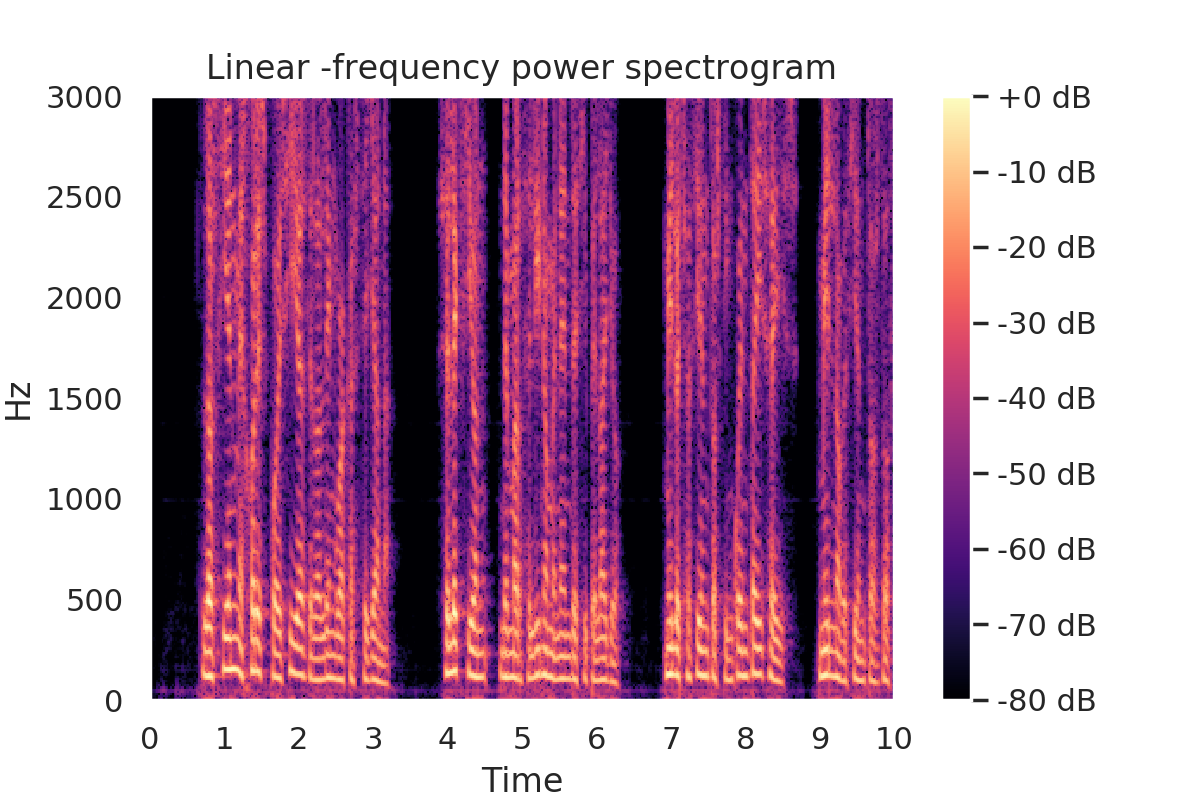
\includegraphics[width=0.9\columnwidth]{figures/audio_book_spectrogram.png}
	\caption{Espectrograma de la voz humana}
	\label{fig: voice_spectral}
\end{figure}

Por el contrario, el ruido blanco cuenta con un ancho banda espectral infinito, i.d., se manifiesta en todas las frecuencias. El ruido de ciudad no es exactamente ruido blanco porque un pitido de un coche sí es una frecuencia característica. En la figura \ref{fig: noise_spectral} se puede ver el espectrograma del ruido de una ciudad. La forma de interpretar el tipo de gráfico es idéntica a la explicada anteriormente. En este caso se ve un espectro más ancho donde predominan las bajas frecuencias y se aprecia algún tipo de ruido que no es de gran ancho de banda, en este caso es una sirena de algún vehículo de emergencias (viene representada por la línea de mayor intensidad cuya frecuencia varía entre 800 Hz y 500 Hz aproximadamente).

\begin{figure}[t!]
	\centering
	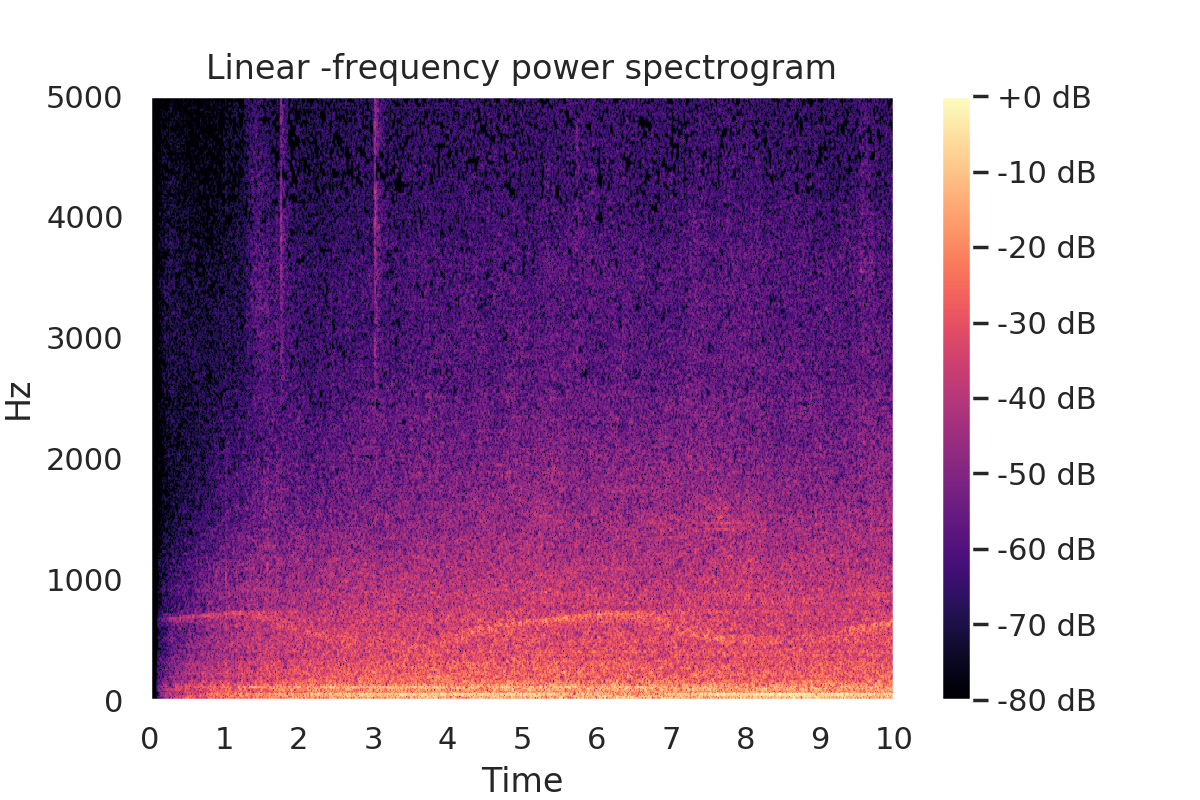
\includegraphics[width=0.9\columnwidth]{figures/noise_spectrogram.png}
	\caption{Espectrograma del ruido}
	\label{fig: noise_spectral}
\end{figure}

Otro tipo de gráfico interesante para analizar es el espectro. El espectro se genera cortando verticalmente el espectrograma. Esto es, un instante de tiempo del espectrograma, de modo que se genera un gráfico bidimensional donde el eje vertical representa la potencia y el horizontal la frecuencia. Otra forma de verlo, sería la inversa, el espectrograma representa la evolución temporal de todos los espectros. Este tipo de gráficos permiten ver las componentes frecuenciales de la voz con más claridad dado que el ruido es constante para todo el ancho de banda. Las gráficas \ref{fig: ffts_audio} y \ref{fig: ffts_noise} representan varios de estos instantes de tiempo superpuestos para cada pista de audio. En la gráfica \ref{fig: ffts_audio} los picos que se aprecian para la curva \textbf{FFT\_35} representan las componentes principales de la voz. Estos picos no van a aparecen en todas las \glspl{FFT} porque la voz es intermitente y además varía de frecuencia a lo largo del tiempo, por eso no se superponen perfectamente para cada \gls{FFT}.

\begin{figure}[h!]
	\centering
	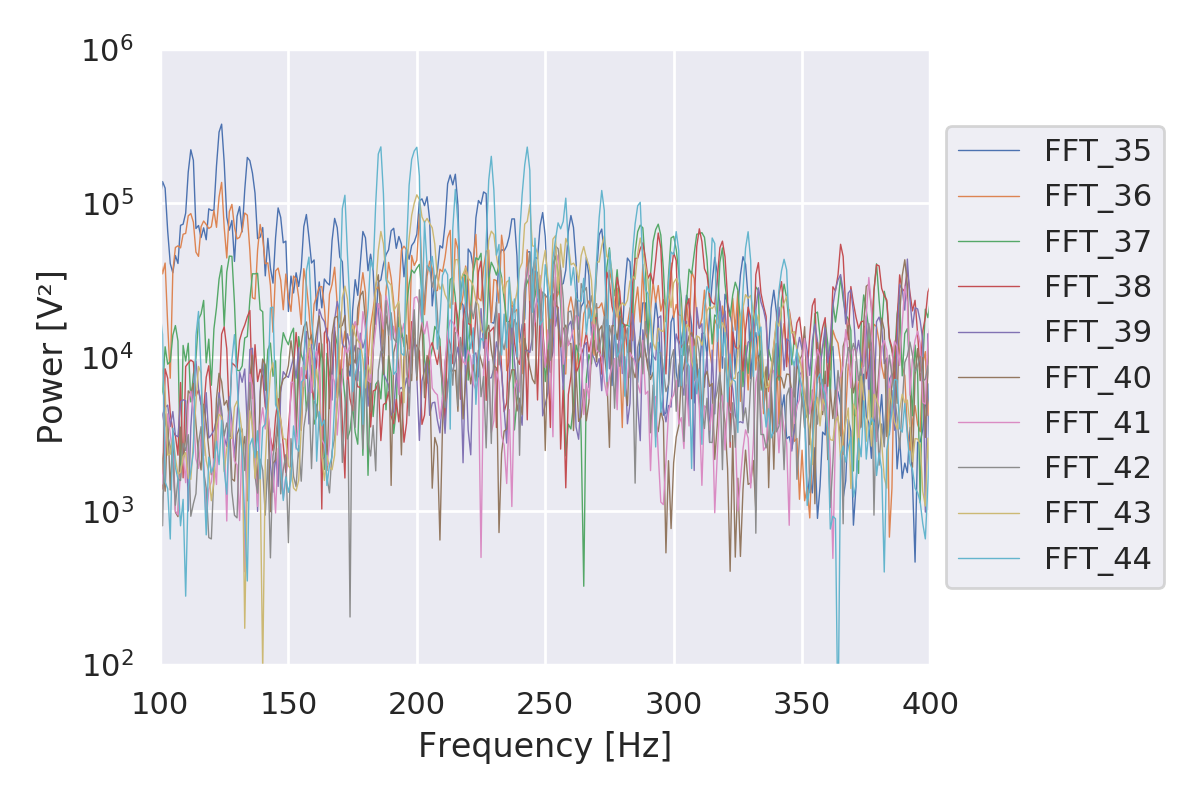
\includegraphics[width=0.9\textwidth]{figures/audio_ffts}
	\caption{10 \acrshort{FFT}s continuas con un overlap del 50\% de la pista de audio}
	\label{fig: ffts_audio}
\end{figure}
\begin{figure}[h!]
	\centering
	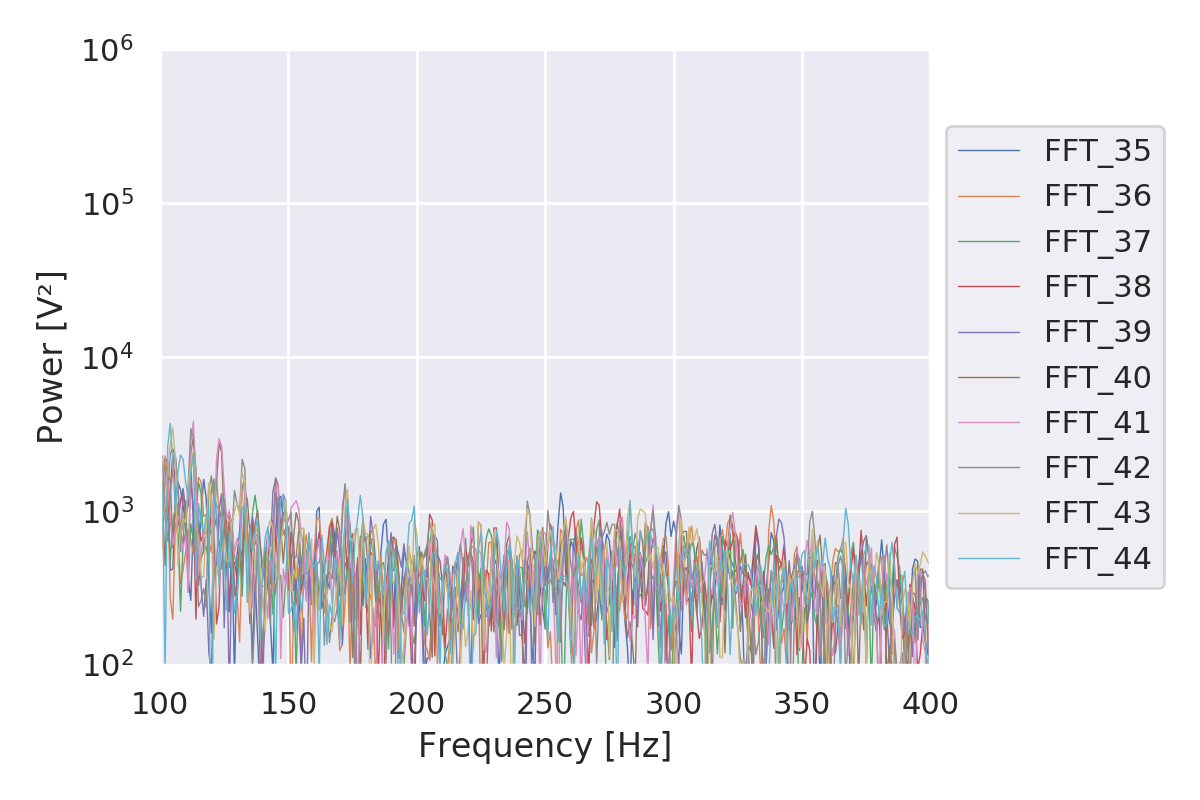
\includegraphics[width=0.9\textwidth]{figures/noise_ffts}
	\caption{10 \acrshort{FFT}s continuas con un overlap del 50\% de la pista de ruido}
	\label{fig: ffts_noise}
\end{figure}

\subsubsection{Combinación de pistas de audio}
El siguiente paso sería analizar el audio como combinación de las pistas de ruido y audiolibro. En la figura \ref{fig: combination_spectral} se puede ver la combinación de ambos audios.

\begin{figure}[h!]
	\centering
	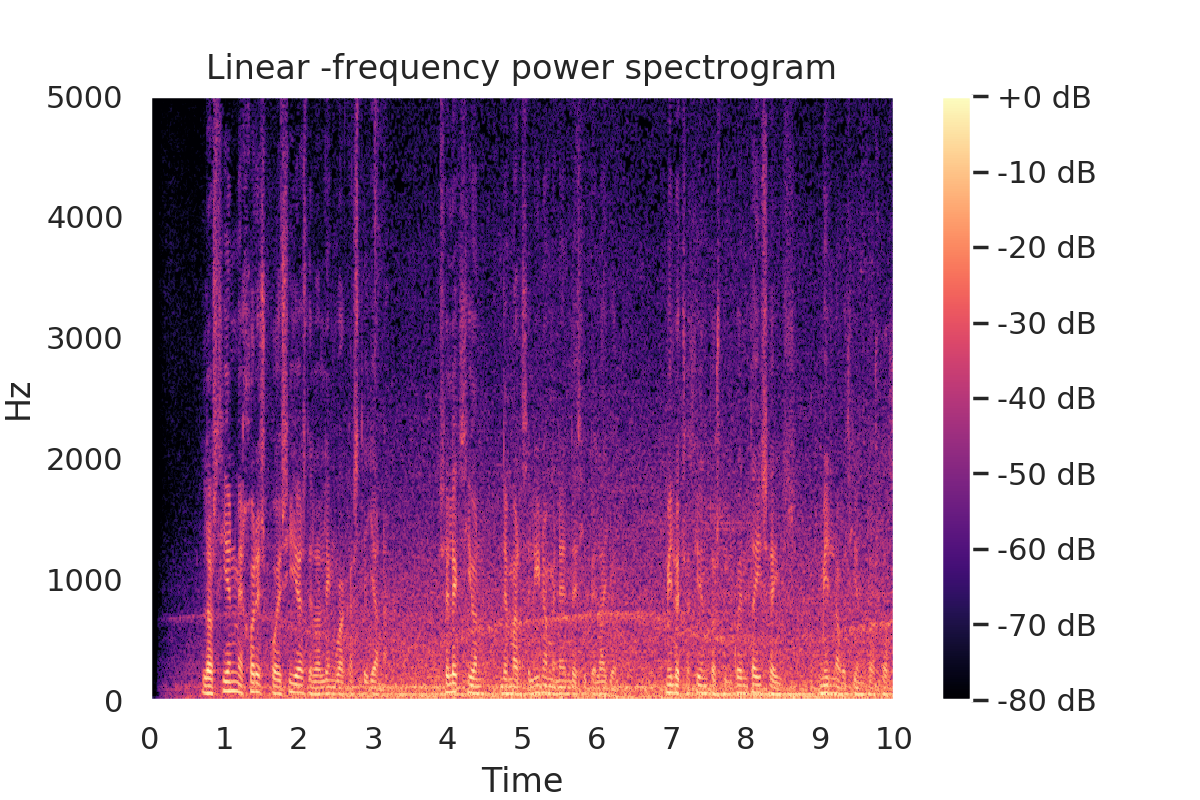
\includegraphics[width=0.9\columnwidth]{figures/combination_spectrogram.png}
	\caption{Espectrograma de las pistas combinadas}
	\label{fig: combination_spectral}
\end{figure}

En este caso la combinación es con los niveles de potencia que tiene cada uno de ellos sin adaptar su amplitud. Idealmente, la combinación de los audios debería ser para un \gls{SNR} dado. Es decir, adaptar las potencias de ruido y audio para que sea cual fuere la combinación de audio y ruido la relación entre señal y ruido fuera la misma. De este modo el algoritmo se entrenaría para un nivel de ruido constante dado un nivel de señal constante, un problema mucho más acotado que dejar libre las potencias de entrada de ruido a audio. Esto no se ha realizado porque se consideraba fuera de la primera aproximación que es lo que este trabajo propone.

Se ha comprobado que la combinación de audio y ruido sea audible y, por consiguiente, el algoritmo pueda discernir entre los niveles de potencia. Esto se demuestra en la figura \ref{fig: combination_spectral} donde aún estando el ruido se pueden distinguir perfectamente las componentes frecuenciales de la voz. Una gráfica interesante es el histograma comparativo entre la señal sin ruido y la combinación de ambas como se muestra en la figura \ref{fig: band0_clean_noisy_hist}. Se puede apreciar que las formas de las distribuciones son similares teniendo la señal libre de ruido más componentes de energía baja, como es de esperar, debido a aquellas bandas en las cuales la persona no habla.

\begin{figure}[h!]
	\centering
	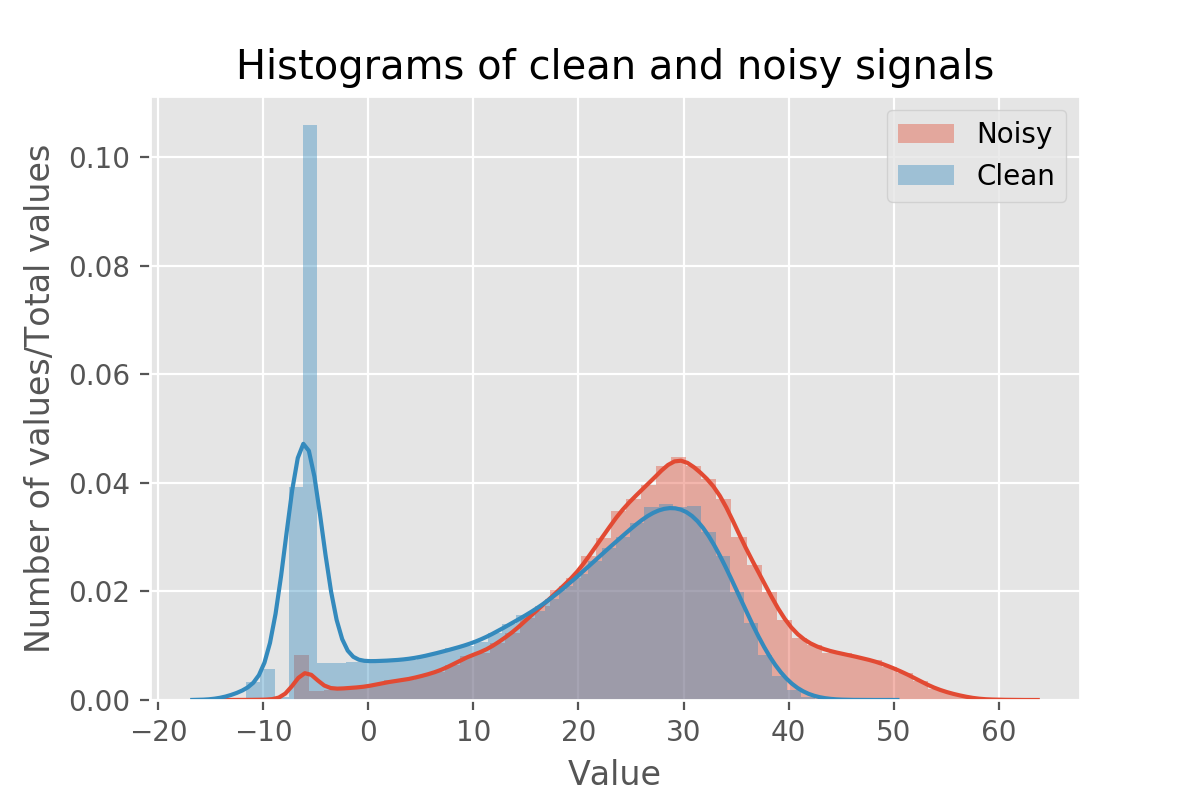
\includegraphics[width=0.6\columnwidth]{figures/band0_clean_noisy_hist.png}
	\caption{Espectrograma de las pistas combinadas}
	\label{fig: band0_clean_noisy_hist}
\end{figure}

\subsubsection{Conclusiones del análisis en el dominio de la frecuencia}
De este breve análisis en el dominio de la frecuencia se pueden extraer varias conclusiones:
\begin{itemize}
	\item \textbf{La voz humana no es continua en el tiempo} (la persona se para para respirar mientras habla) lo que crea un espectro seccionado en el tiempo. Por el contrario el \textbf{ruido sí es continuo en el tiempo}.\footnote{Esta conclusión se verá también en el dominio del tiempo donde la amplitud de la señal cae para el audio humano.}
	\item El \textbf{espectro de la voz humana está acotado en frecuencia} mientras que el espectro del ruido, en general, no. Como implicación directa tiene que para analizar el audio en el dominio de la frecuencia se puede acotar la tasa de muestreo a la banda donde la voz humana se encuentra, ahorrando mucho procesado.
	\item La \textbf{voz humana} se caracteriza por tener unas \textbf{frecuencias características} que varían en el tiempo y están relacionadas entre sí (tono fundamental y armónicos). Por el contrario el ruido, no presenta relación entre sus componentes espectrales.
	\item Tras la combinación de los audios, si las amplitudes del ruido no son lo suficientemente grandes, las componentes frecuenciales de la voz siguen siendo predominantes en el espectrograma.
\end{itemize}

\subsection{Dominio del tiempo}
En el dominio del tiempo analizar una señal de tan alta tasa de muestreo es algo complicado. Es mucho más interesante estudiar la envuelta de la señal. En las figuras \ref{fig: voice_time} y \ref{fig: noise_time} se pueden ver las envueltas de las señales de audio y ruido respectivamente. En primer lugar se aprecia, al igual que en el espectro, que la voz es intermitente en el tiempo, existiendo pausas cortas y largas. Otro punto a destacar son las amplitudes, la del ruido es mucho menor, lo que va a permitir que al combinar ambos audios, el audio no se enmascare detrás del ruido como se ve en la figura \ref{fig: combination_time}.

\begin{figure*}[h!]
	\centering
	\begin{subfigure}[t]{0.5\textwidth}
		\centering
		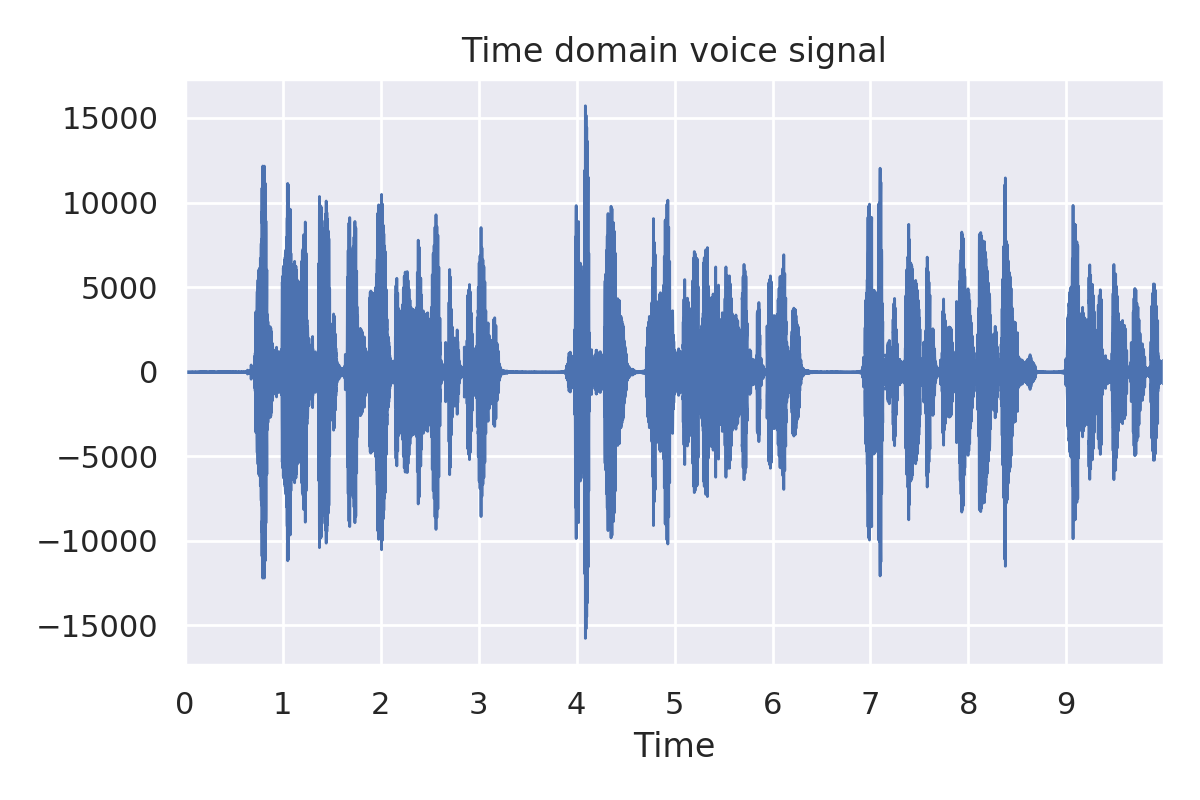
\includegraphics[width=0.9\columnwidth]{figures/audio_book_time.png}
		\caption{Forma de la señal de audio en el dominio del tiempo}
		\label{fig: voice_time}
	\end{subfigure}%
	\hspace*{10pt}
	\begin{subfigure}[t]{0.5\textwidth}
		\centering
		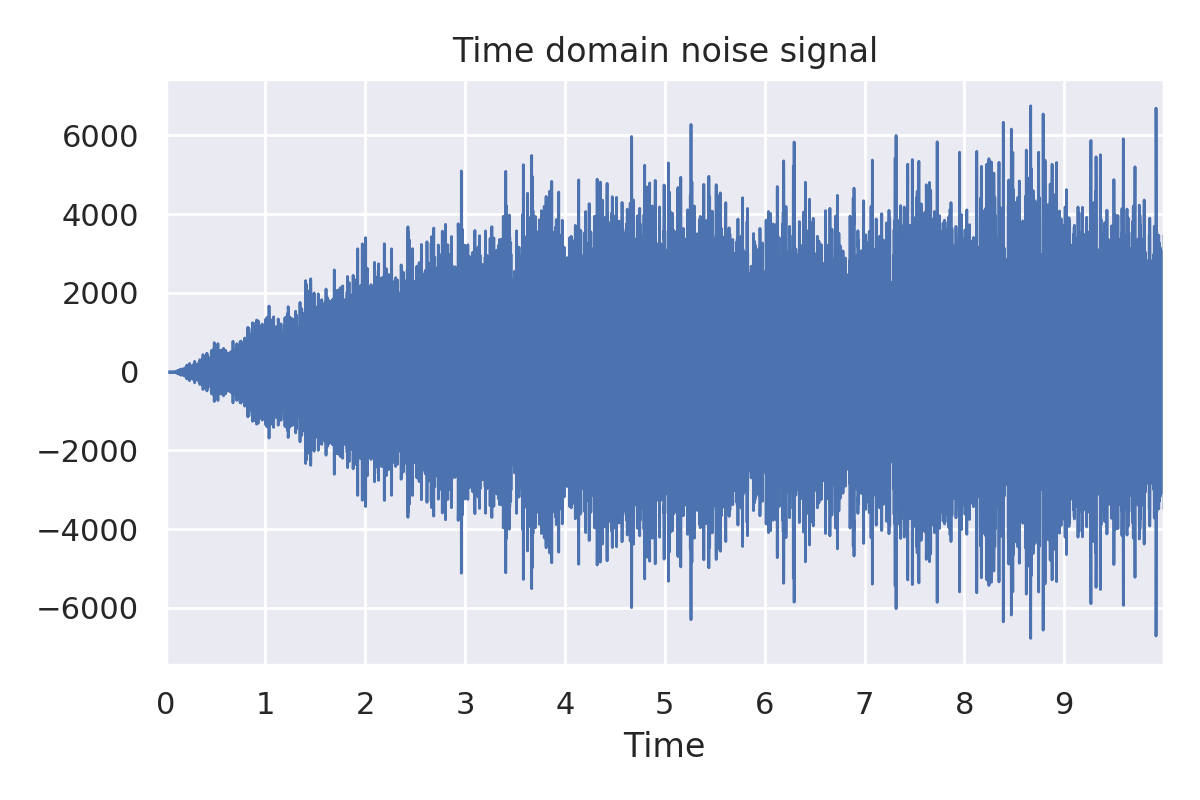
\includegraphics[width=0.9\columnwidth]{figures/noise_time.png}
		\caption{Forma de la señal de ruido en el dominio del tiempo}
		\label{fig: noise_time}
	\end{subfigure}
	\caption{Series temporales de las pistas de audio y ruido}
\end{figure*}
\begin{figure*}[h!]
	\centering
	\begin{subfigure}[t]{0.5\textwidth}
		\centering
		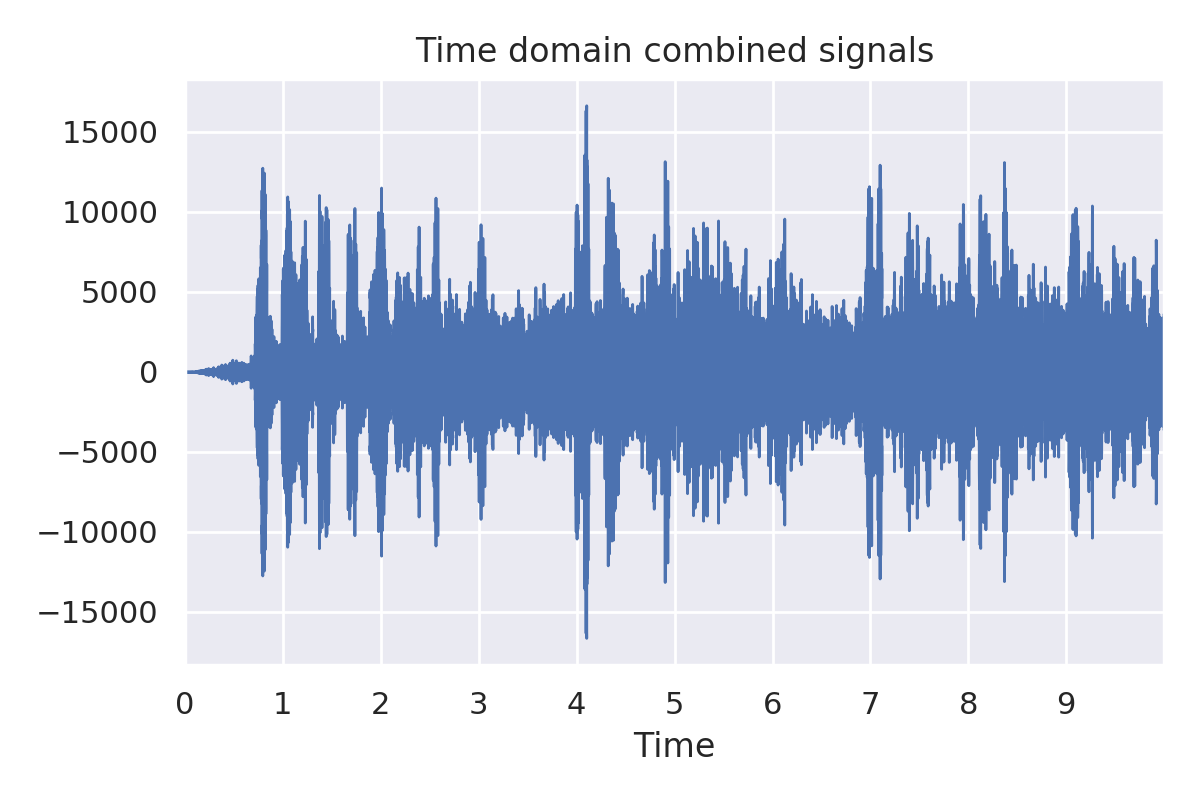
\includegraphics[width=\columnwidth]{figures/combination_time.png}
		\caption{Forma de la señal combinada de audio y ruido en el dominio del tiempo}
		\label{fig: combination_time}
	\end{subfigure}%
	\hspace*{10pt}
	\begin{subfigure}[t]{0.5\textwidth}
		\centering
		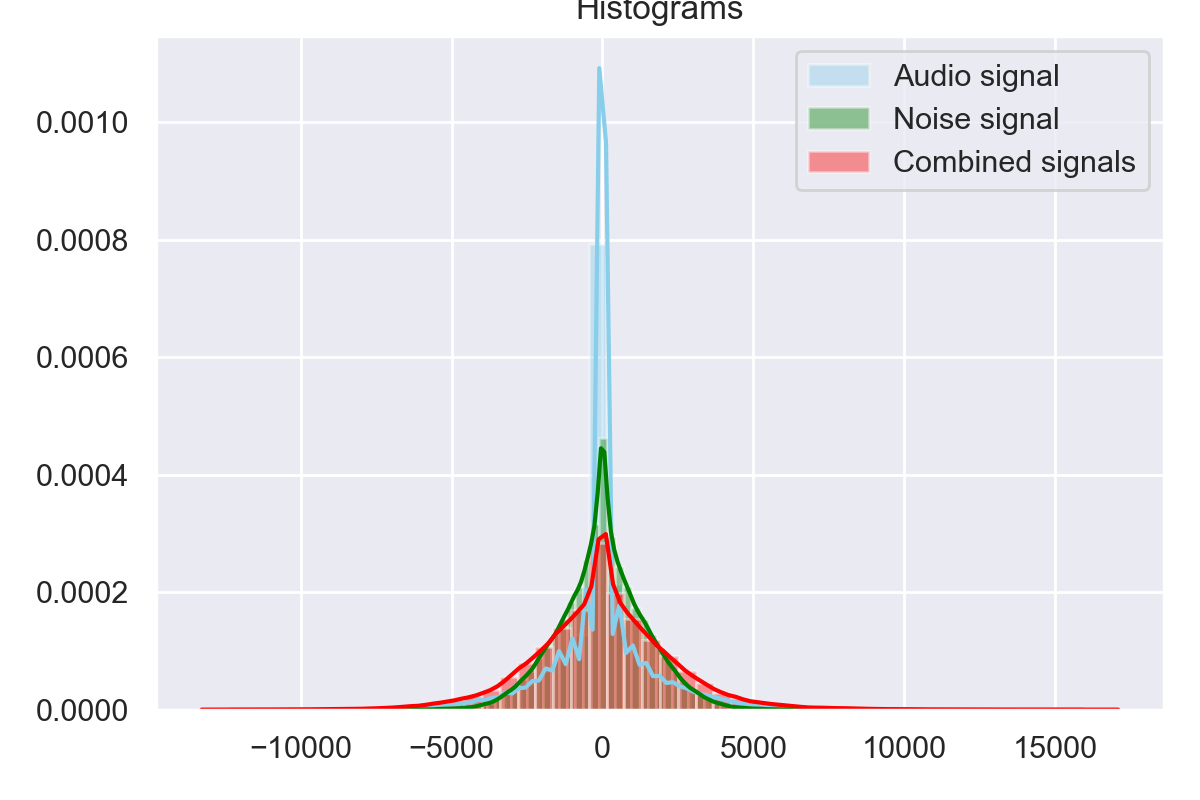
\includegraphics[width=\columnwidth]{figures/hist_time.png}
		\caption{Histogramas superpuestos de las tres señales}
		\label{fig: hist_time}
	\end{subfigure}
	\caption{Serie temporal del audio combinado y comparativa de los histogramas en el dominio del tiempo}
\end{figure*}

Otro aspecto interesante de las señales sería estudiar su histograma. En la figura \ref{fig: hist_time} se pueden ver los histogramas de las tres señales. Las conclusiones que se pueden extraer es que las tres señales están centradas en cero, algo lógico debido a la naturaleza de la medida, el audio es una onda de presión. La tres distribuciones son muy parecidas y no es útil usar el histograma para pasar de una distribución a otra.